%%%%%%%%%%%%%%%%%%%%%%%%%%%%% Define Article %%%%%%%%%%%%%%%%%%%%%%%%%%%%%%%%%%
\documentclass{article}
%%%%%%%%%%%%%%%%%%%%%%%%%%%%%%%%%%%%%%%%%%%%%%%%%%%%%%%%%%%%%%%%%%%%%%%%%%%%%%%

%%%%%%%%%%%%%%%%%%%%%%%%%%%%% Using Packages %%%%%%%%%%%%%%%%%%%%%%%%%%%%%%%%%%
\usepackage{geometry}
\usepackage{graphicx}
\usepackage{amssymb}
\usepackage{amsmath}
\usepackage{amsthm}
\usepackage{empheq}
\usepackage{mdframed}
\usepackage{booktabs}
\usepackage{lipsum}
\usepackage{graphicx}
\usepackage{color}
\usepackage{psfrag}
\usepackage{pgfplots}
\usepackage{bm}
%%%%%%%%%%%%%%%%%%%%%%%%%%%%%%%%%%%%%%%%%%%%%%%%%%%%%%%%%%%%%%%%%%%%%%%%%%%%%%%

% Other Settings

%%%%%%%%%%%%%%%%%%%%%%%%%% Page Setting %%%%%%%%%%%%%%%%%%%%%%%%%%%%%%%%%%%%%%%
\geometry{a4paper}

%%%%%%%%%%%%%%%%%%%%%%%%%% Define some useful colors %%%%%%%%%%%%%%%%%%%%%%%%%%
\definecolor{ocre}{RGB}{243,102,25}
\definecolor{mygray}{RGB}{243,243,244}
\definecolor{deepGreen}{RGB}{26,111,0}
\definecolor{shallowGreen}{RGB}{235,255,255}
\definecolor{deepBlue}{RGB}{61,124,222}
\definecolor{shallowBlue}{RGB}{235,249,255}
%%%%%%%%%%%%%%%%%%%%%%%%%%%%%%%%%%%%%%%%%%%%%%%%%%%%%%%%%%%%%%%%%%%%%%%%%%%%%%%

%%%%%%%%%%%%%%%%%%%%%%%%%% Define an orangebox command %%%%%%%%%%%%%%%%%%%%%%%%
\newcommand\orangebox[1]{\fcolorbox{ocre}{mygray}{\hspace{1em}#1\hspace{1em}}}
%%%%%%%%%%%%%%%%%%%%%%%%%%%%%%%%%%%%%%%%%%%%%%%%%%%%%%%%%%%%%%%%%%%%%%%%%%%%%%%

%%%%%%%%%%%%%%%%%%%%%%%%%%%% English Environments %%%%%%%%%%%%%%%%%%%%%%%%%%%%%
\newtheoremstyle{mytheoremstyle}{3pt}{3pt}{\normalfont}{0cm}{\rmfamily\bfseries}{}{1em}{{\color{black}\thmname{#1}~\thmnumber{#2}}\thmnote{\,--\,#3}}
\newtheoremstyle{myproblemstyle}{3pt}{3pt}{\normalfont}{0cm}{\rmfamily\bfseries}{}{1em}{{\color{black}\thmname{#1}~\thmnumber{#2}}\thmnote{\,--\,#3}}
\theoremstyle{mytheoremstyle}
\newmdtheoremenv[linewidth=1pt,backgroundcolor=shallowGreen,linecolor=deepGreen,leftmargin=0pt,innerleftmargin=20pt,innerrightmargin=20pt,]{theorem}{Theorem}[section]
\theoremstyle{mytheoremstyle}
\newmdtheoremenv[linewidth=1pt,backgroundcolor=shallowBlue,linecolor=deepBlue,leftmargin=0pt,innerleftmargin=20pt,innerrightmargin=20pt,]{definition}{Definition}[section]
\theoremstyle{myproblemstyle}
\newmdtheoremenv[linecolor=black,leftmargin=0pt,innerleftmargin=10pt,innerrightmargin=10pt,]{problem}{Problem}[section]
%%%%%%%%%%%%%%%%%%%%%%%%%%%%%%%%%%%%%%%%%%%%%%%%%%%%%%%%%%%%%%%%%%%%%%%%%%%%%%%

%%%%%%%%%%%%%%%%%%%%%%%%%%%%%%% Plotting Settings %%%%%%%%%%%%%%%%%%%%%%%%%%%%%
\usepgfplotslibrary{colorbrewer}
\pgfplotsset{width=8cm,compat=1.9}
\parindent=0pt
\parskip=5pt
%%%%%%%%%%%%%%%%%%%%%%%%%%%%%%%%%%%%%%%%%%%%%%%%%%%%%%%%%%%%%%%%%%%%%%%%%%%%%%%

%%%%%%%%%%%%%%%%%%%%%%%%%%%%%%% Title & Author %%%%%%%%%%%%%%%%%%%%%%%%%%%%%%%%
\title{IMO Shortlist Writeups}
\author{Alston Yam}
%%%%%%%%%%%%%%%%%%%%%%%%%%%%%%%%%%%%%%%%%%%%%%%%%%%%%%%%%%%%%%%%%%%%%%%%%%%%%%%


\begin{document}
    \maketitle
    \section{Introduction}
    Here's a compiled list of my typed up solutions to various IMO shortlist problems during my preparation for the 66th IMO.
    
    \section{Problems}
    \subsection{ISL 2022}

    \begin{problem}[2022 A1]
        Let $(a_n)_{n\geq 1}$ be a sequence of positive real numbers with the property that
            \[ (a_{n+1})^2 + a_na_{n+2} \leq a_n + a_{n+2} \]
        for all positive integers $n$. Show that $a_{2022}\leq 1$.
    \end{problem}

    \begin{proof}[Solution]
        Define a sequence $b_i = a_i - 1$ $\forall i$. The given condition is equivalent to \[b_nb_{n+2} + b_{n+1}(b_{n+1} + 2) \leq 0\]
        Where $b_i > -1$ $\forall i$. Now FTSOC $b_{2022} > 0$. Notice we also have \[b_{n-1}b_{n+1} + b_{n}(b_{n} + 2) \leq 0\]
        Summing the two gives
        \[b_n(b_{n-1} + b_n + 2) + b_{n+1}(b_{n+1} + b_{n-1} + 2)\leq 0\]
        Substituting $n=2022$ and $n=2021$ into the above eqeuation, we get that $b_{2021} < 0$ and also $b_{2023} < 0$ respectively. As a result, considering $n=2021$ in the first equation gives us a contradiction, and we're done.
    \end{proof}

    \subsection{ISL 2019}

    \begin{problem}[2019 G4]
        Let $P$ be a point inside triangle $ABC$. Let $AP$ meet $BC$ at $A_1$, let $BP$ meet $CA$ at $B_1$, and let $CP$ meet $AB$ at $C_1$. Let $A_2$ be the point such that $A_1$ is the midpoint of $PA_2$, let $B_2$ be the point such that $B_1$ is the midpoint of $PB_2$, and let $C_2$ be the point such that $C_1$ is the midpoint of $PC_2$. Prove that points $A_2, B_2$, and $C_2$ cannot all lie strictly inside the circumcircle of triangle $ABC$.
    \end{problem}


    \begin{center}
        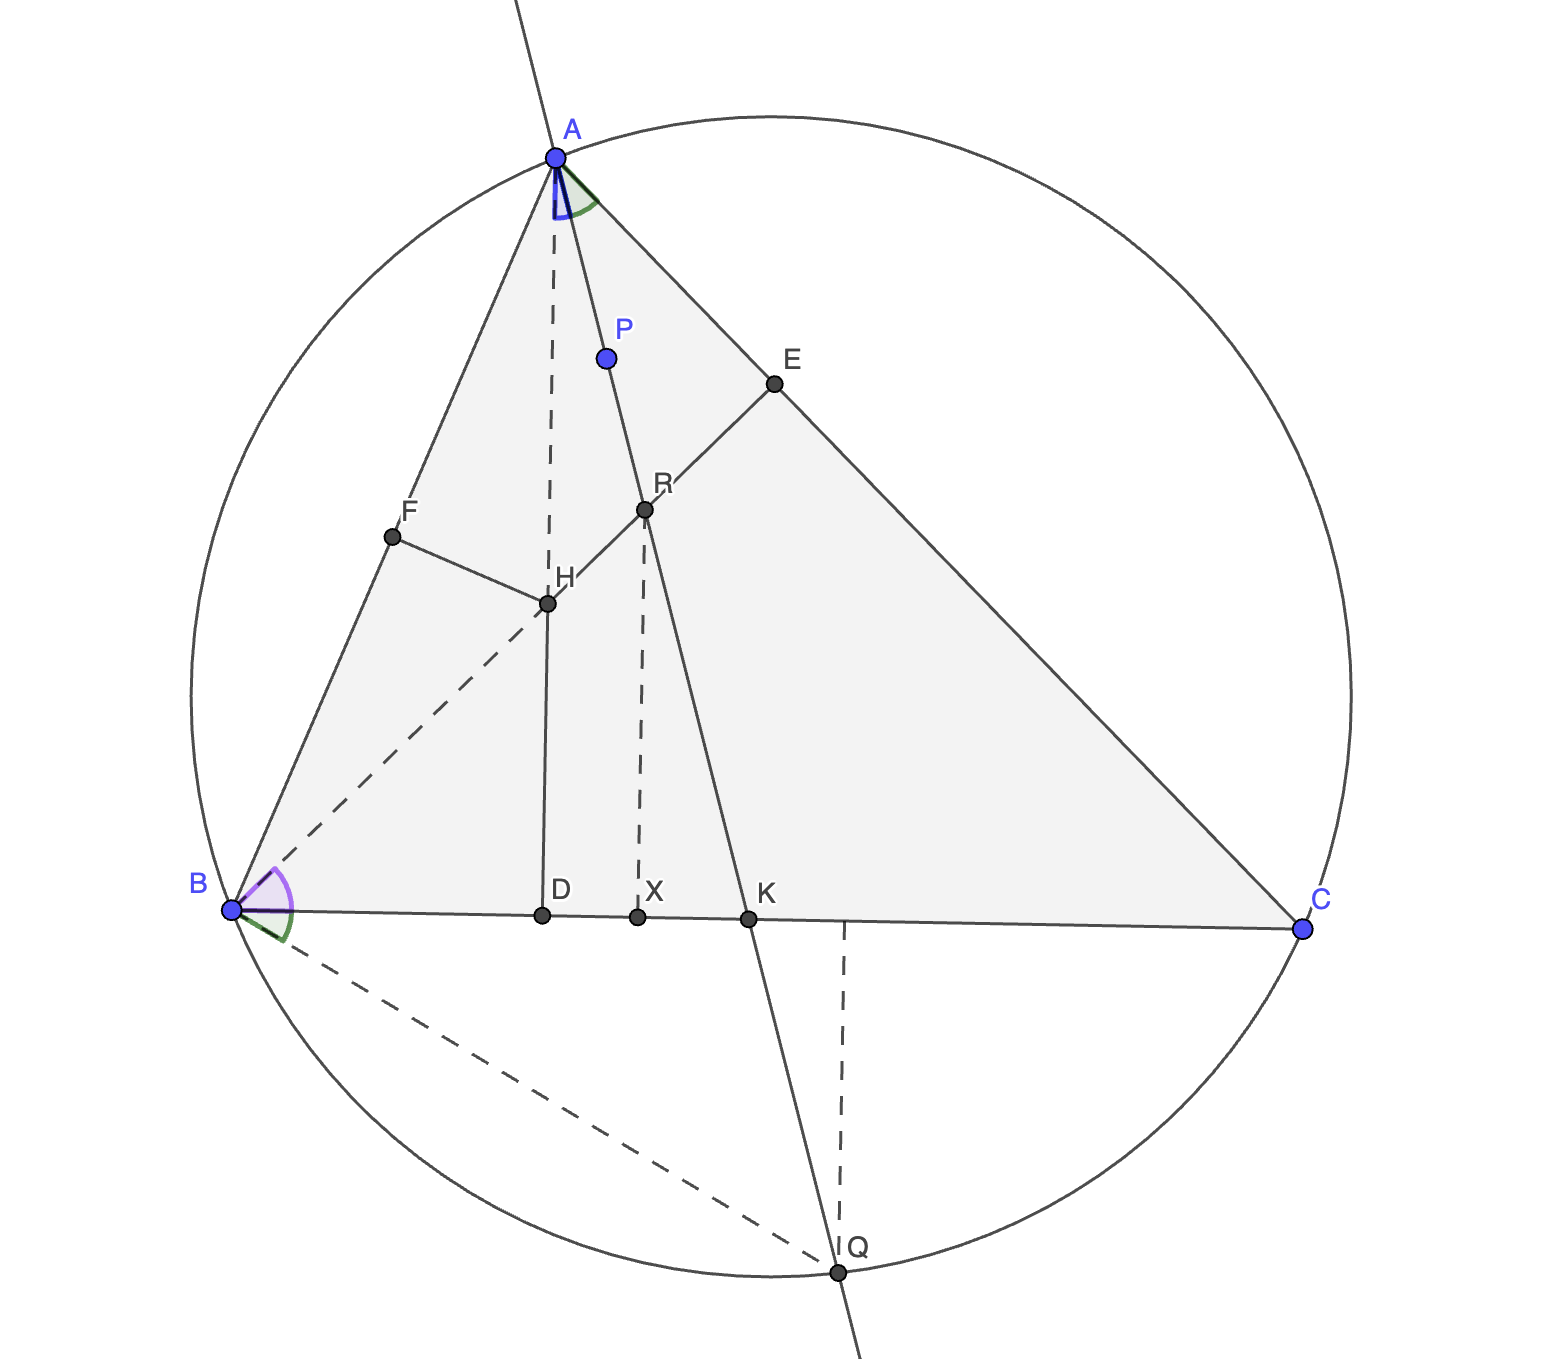
\includegraphics[scale=0.4]{2019 G4.png}

        \textit{Fig 1: Diagram for 2019 G4}
    \end{center}

    \begin{proof}
        We will first prove the case where $ABC$ is acute, and then deal with the obtuse case.
    \end{proof}

    \textbf{Remark:} As I was attempting this problem, I told myself that barycentric coordinates would be an easy way to solve this, but I didn't know how they worked :( It turns out, this problem is much easier with a bary bash. 

    \begin{problem}[2019 N3]
        We say that a set $S$ of integers is \textit{rootiful} if, for any positive integer $n$ and any $a_0, a_1, \cdots, a_n \in S$, all integer roots of the polynomial $a_0+a_1x+\cdots+a_nx^n$ are also in $S$. Find all rootiful sets of integers that contain all numbers of the form $2^a - 2^b$ for positive integers $a$ and $b$.
    \end{problem}

    \begin{proof}
        I claim that the answer is $S \in \mathbb{Z}$. Clearly this works. Now we prove that if we start with the set $S = \{2^a - 2^b \mid a, b \in \mathbb{Z}^+\}$, we can then get every integer with the appropriate choices of coefficients. 
        
        First we see $1$ is in S by taking $P(x) = 2x - 2$.

        Now, notice that if $k$ is in $S$, $-k$ must also be in $S$ by taking $P(x) = x + k$. Therefore, we restrict our search to only positive integers, as the negative integers will follow.

        We will take the minimal positive integer $m$ such that $m \notin S$ and aim to find a contradiction. Let $m = 2^ep$, where $p$ is odd. Consider the number $M = 2^{e + \varphi(p) + 1} - 2^{e+1} = 2^{e+1}(2^{\varphi(p)} - 1)$. Clearly $M \in S$ and $m \mid M$ (by Euler's Theorem).
        
        We write $M = b_1m + b_2m^2 + b_3m^3 + \cdots + b_nm^n$. Then we can consider the polynomial \[P(x) = -M + b_1x + b_2x^2 + b_3x^3 + \cdots + b_nx^n\]

        This works as $b_i \in S$ $\forall i$ since $b_i < m$. Finally, notice that $m$ must be a root to the above polynomial, and so $m \in S$, and we're done.
    \end{proof}

    
    \subsection{ISL 2017}
    \begin{problem}[2017 A4]
        A sequence of real numbers $a_1,a_2,\ldots$ satisfies the relation
\[ a_n=-\max_{i+j=n}(a_i+a_j)\qquad\text{for all}\quad n>2017. \]
Prove that the sequence is bounded, i.e., there is a constant $M$ such that $|a_n|\leq M$ for all positive integers $n$.
    \end{problem}

    \begin{proof}

Let's denote $a_x$ to be the element with the maximum absolute value in the set $\{a_1, a_2, \cdots a_{2017}\}$. We split the problem into cases:

\textcolor{red}{Case 1}: $a_x = 0$. This case is trivial as all values in the sequence is equal to $0$.
\vspace{5pt}

\textcolor{red}{Case 2}: $a_x > 0$. Let $M = a_x$, I will prove that $-2M \leq a_i \leq M$ $\forall i$.
Proof: Notice that $$\max_{i+j=2018}(a_i+a_j) \geq a_{x} + a_{2018 - x} \geq 0$$
So $a_{2018} = -\max_{i+j=2018}(a_i+a_j) \leq 0$, i.e. It's bounded above by 0.
We also know that $$\max_{i+j=2018}(a_i+a_j) \leq M + M = 2M$$ so $a_{2018} = - \max_{i+j=2018}(a_i+a_j) \geq -2M$. So we have $$-2M \leq a_{2018} \leq 0$$
Now, if $-M \leq a_{2018} \leq 0$, we can carry on this process iteratively to get that the next element also has the bound stated above. Otherwise, assume that $-2M \leq a_{2018} < -M$. We see that $$\max_{i+j=2019}(a_i+a_j) \geq a_x + a_{2019-x} \geq M + (-2M) = -M$$
So that means $a_{2019} = -\max_{i+j=2019}(a_i+a_j) \leq M$. But also, $$\max_{i+j=2019}(a_i+a_j) \leq M + M = 2M$$
    
So we have $$-2M \leq a_{2019} \leq M$$

Thus we may continue this process iteratively to get that $-2M \leq a_i \leq M$ $\forall i$.



\textcolor{red}{Case 3}: $a_x < 0$. Let $-M = a_x$, $M > 0$. 

Notice that $$\max_{i+j=2018}(a_i+a_j) \leq 2M$$
$$\max_{i+j=2018}(a_i+a_j) \geq -2M$$

So we achieve the bound that $-2M \leq a_{2018} \leq 2M$. 


\textcolor{pink}{Case 3.1}: If $M < a_{2018} \leq 2M$, we can refer to Case 2 above to see that the sequence is bounded.

\textcolor{pink}{Case 3.2}: If $-M \leq a_{2018} \leq M$, We can iterate this process again, as $a_x = -M$ is still the $a_i$ with the largest absolute value. 


\textcolor{pink}{Case 3.3}: $-2M \leq a_{2018} < -M$.

Let $a_{2018} = -k$. Therefore there must exist $p, q$ such that $p + q = 2018$ and $a_p + a_q = k$. WLOG let $a_p \geq \frac{k}{2}$.

We see $$\max_{i+j=2019}(a_i+a_j) \geq a_p + a_{2019 - p} \geq \frac{k}{2} + (-k) = \frac{-k}{2} \geq \frac{-2M}{2} = -M$$
and also $$\max_{i+j=2019}(a_i+a_j) \leq M + M = 2M$$ So we actually see that 
$$-2M \leq a_{2019} \leq M$$

But we're done here, by considering the most negative element $a_n = -N$. There must be an $a_i$ with $a_i > \frac{N}{2}$, so the lower bound for $\max_{i+j=n}(a_i+a_j)$ is $\frac{N}{2} + (-N) = \frac{-N}{2} \geq -M$. The upper bound of $2M$ is obvious to see.

So when when calculate the next values of the sequence, the upper and lower bounds for $\max_{i+j=n}(a_i+a_j)$ are fixed at $2M$ and $-M$ respectively, so we're done.


    \end{proof}
\end{document}